\documentclass[11pt]{article}

% Change "review" to "final" for a camera-ready version.
\usepackage[preprint]{acl}
% \makeatletter
% \acl@anonymizefalse
% \makeatother

\usepackage{times}
\usepackage{latexsym}
\usepackage[T1]{fontenc}
\usepackage[utf8]{inputenc}
\usepackage{microtype}
% \usepackage{inconsolata} % optional; unavailable in some cluster TeX installs
\usepackage{graphicx}
\usepackage{booktabs}
\usepackage{multirow}
\usepackage{tabularx}
\usepackage{amsmath}
\usepackage{xcolor}
\usepackage{listings}
\usepackage{enumitem}
\usepackage{xspace}

\newcommand{\sys}{GLOBALNAV\xspace}
\newcommand{\bench}{GlobNav-Bench\xspace}

\lstdefinestyle{promptstyle}{
  basicstyle=\ttfamily\scriptsize,
  breaklines=true,
  breakatwhitespace=false,
  columns=fullflexible,
  keepspaces=true,
  showstringspaces=false,
  frame=single,
  framerule=0.3pt,
  framesep=3pt,
  backgroundcolor=\color{gray!5},
  rulecolor=\color{gray!45},
  aboveskip=0.5em,
  belowskip=0.5em
}


\newcommand{\placeholder}[1]{%
  \begin{center}
    \fbox{\begin{minipage}{0.92\linewidth}
      \centering \vspace{0.7em}
      \textit{#1}
      \vspace{0.7em}
    \end{minipage}}
  \end{center}
}

\title{\sys: An Environment-Driven Agent for Global Multimodal Route Planning}

\author{
  Shunfeng Zheng$^{1}$, Meng Fang$^{2}$, Ling Chen$^{1}$ \\
  $^{1}$University of Technology Sydney, New South Wales, Australia \\
  $^{2}$University of Liverpool, Liverpool, the United Kingdom \\
  \texttt{Shunfeng.Zheng@student.uts.edu.au} \\
  \texttt{Meng.Fang@liverpool.ac.uk, Ling.Chen@uts.edu.au}
}

\begin{document}
\maketitle

\begin{abstract}
Real-world travel requests are often global, multi-modal, and interactive: a user may ask for a trip that combines local access, long-distance transportation, ground transfers, and clarification of underspecified endpoints. We present \sys, an LLM-based system that uses an LLM for intent extraction and ambiguity clarification, while a routing backend generates route options from OpenStreetMap, OpenFlights, Overpass, and mode-specific graph search. \sys presents segment-level route alternatives in an interactive interface, allowing users to inspect, compare, and revise walking, driving, public-transit, flight, ferry, and transfer options. We also introduce \bench, a 100-example benchmark for evaluating system-level success in global multi-modal route planning, focusing on whether the system resolves user requests and returns grounded travel solutions. Across \bench and 1,723 external route-request instances derived from MultiWOZ 2.4, Schema-Guided Dialogue, and ATIS, we evaluate \sys, with the deployed GPT-4.1 mini configuration achieving 97\% system success on \bench and 97.4\% on the external set. \sys is available at \url{https://sites.google.com/view/globalnav/home}.




\end{abstract}

\section{Introduction}

Real-world travel planning is rarely a single-mode shortest-path problem~\citep{bast-etal-2016-route-planning}. A user may ask for a trip that combines walking to a station, taking public transit to an airport, flying to another city, and choosing between a taxi, ferry, or walking route for the final segment. The same user may also express personal preferences, such as avoiding driving, preferring a scenic ferry, minimizing transfers, or asking for a cheaper public-transport option. As AI assistants become a more natural interface for everyday services~\citep{rastogi-etal-2020-schema}, navigation systems increasingly need to recover structured travel intent from informal, underspecified language rather than from pre-filled forms~\citep{hemphill-etal-1990-atis}. A practical system must therefore (i) extract origins, destinations, and constraints from free-form user requests; (ii) ask targeted clarification questions when endpoints are missing or ambiguous; (iii) determine transportation modes from map and transport data rather than language priors alone; and (iv) expose alternative segment-level choices to the user, since the ``best'' route is often subjective.


Large language models (LLMs) have advanced rapidly as general-purpose language interfaces: scaling improves few-shot task adaptation~\citep{NEURIPS2020_1457c0d6}, chain-of-thought prompting improves multi-step reasoning~\citep{NEURIPS2022_9d560961}, and recent work explicitly studies their spatial-reasoning and path-generation capabilities~\citep{rizvi-etal-2024-sparc}. However, existing route-planning interfaces and LLM assistants still leave a gap between natural language travel intent and grounded multi-modal routes. Conventional map interfaces are strong once the origin, destination, and mode are specified, but they usually assume that the user has already resolved ambiguous places, decomposed a complex trip into stages, and chosen which transportation modes to compare. Recent language-agent travel-planning benchmarks similarly show that LLM agents struggle with tool use and constraint tracking in realistic travel tasks~\citep{pmlr-v235-xie24j}. Pure LLM planning, by contrast, can produce fluent itineraries but cannot by itself guarantee that an airport transfer, ferry leg, road segment, or public-transit option is supported by external mobility evidence.

To address these requirements, we introduce \sys, an LLM-based, environment-driven demo for global route planning. \sys uses the LLM for language-facing operations, including intent parsing, ambiguity clarification, and high-level route explanation, while route construction and travel options are determined by a routing environment. For local and access segments, the environment constructs route candidates from OSRM road routes, OSM/Overpass stops and route relations, and walking transfers~\citep{Haklay_2008,luxen-vetter-2011}. It returns a driving option when the road network supports one, preserves a pure walking option as a mandatory reference, and exposes alternative routes according to travel time and user preferences. For long-range segments, the environment connects local access and egress segments with verified long-distance connectivity: OpenFlights provides air-route connectivity~\citep{openflights_data_2026}, while ferry/maritime legs are grounded by OSM/Overpass ferry-terminal and port evidence. The same route-option layer also supports bus, train, and tram alternatives for access and egress using OSM/Overpass stops, route relations, and walking-transfer links. We evaluate the deployed GPT-4.1 mini configuration on \bench and on 1,723 OD-eligible route-request examples derived from MultiWOZ 2.4~\citep{ye-etal-2022-multiwoz}, Schema-Guided Dialogue (SGD)~\citep{rastogi-etal-2020-schema}, and ATIS~\citep{hemphill-etal-1990-atis}. \sys reaches 97\% system success rate (SSR) on \bench and 97.4\% SSR on the external set, with 99.4\% Ask/Act accuracy and 98.4\% accuracy for both origin and destination resolution.

This paper makes three contributions:
\begin{enumerate}[leftmargin=*]
\item We introduce \sys, an environment-driven global multi-modal route-planning demo that uses LLMs for language understanding and clarification while grounding route options in an external mobility environment.
\item We construct \bench, a benchmark with an annotation protocol for evaluating global multi-modal navigation requests, covering intent parsing, ambiguity clarification, and environment-grounded route generation.
\item We provide a focused system-level evaluation of the demo on \bench, plus an external origin--destination parsing evaluation over MultiWOZ 2.4, SGD, and ATIS.
\end{enumerate}


\section{GLOBALNAV}
\label{sec:system}

\subsection{User Interaction Flow}

\sys is implemented as an interactive web demo for language-driven global route planning. A user enters a free-form travel request in the browser interface, and the backend first resolves the language-facing parts of the request before invoking the routing environment. The system is organized around three components: an intent parser and clarifier, a mobility environment, and an interactive GUI. The LLM handles user-facing language operations, including intent interpretation, ambiguity detection, clarification questions, and high-level route explanation, while the environment grounds the request in geographic and transportation data and constructs route options.

\begin{figure*}[ht]
\centering
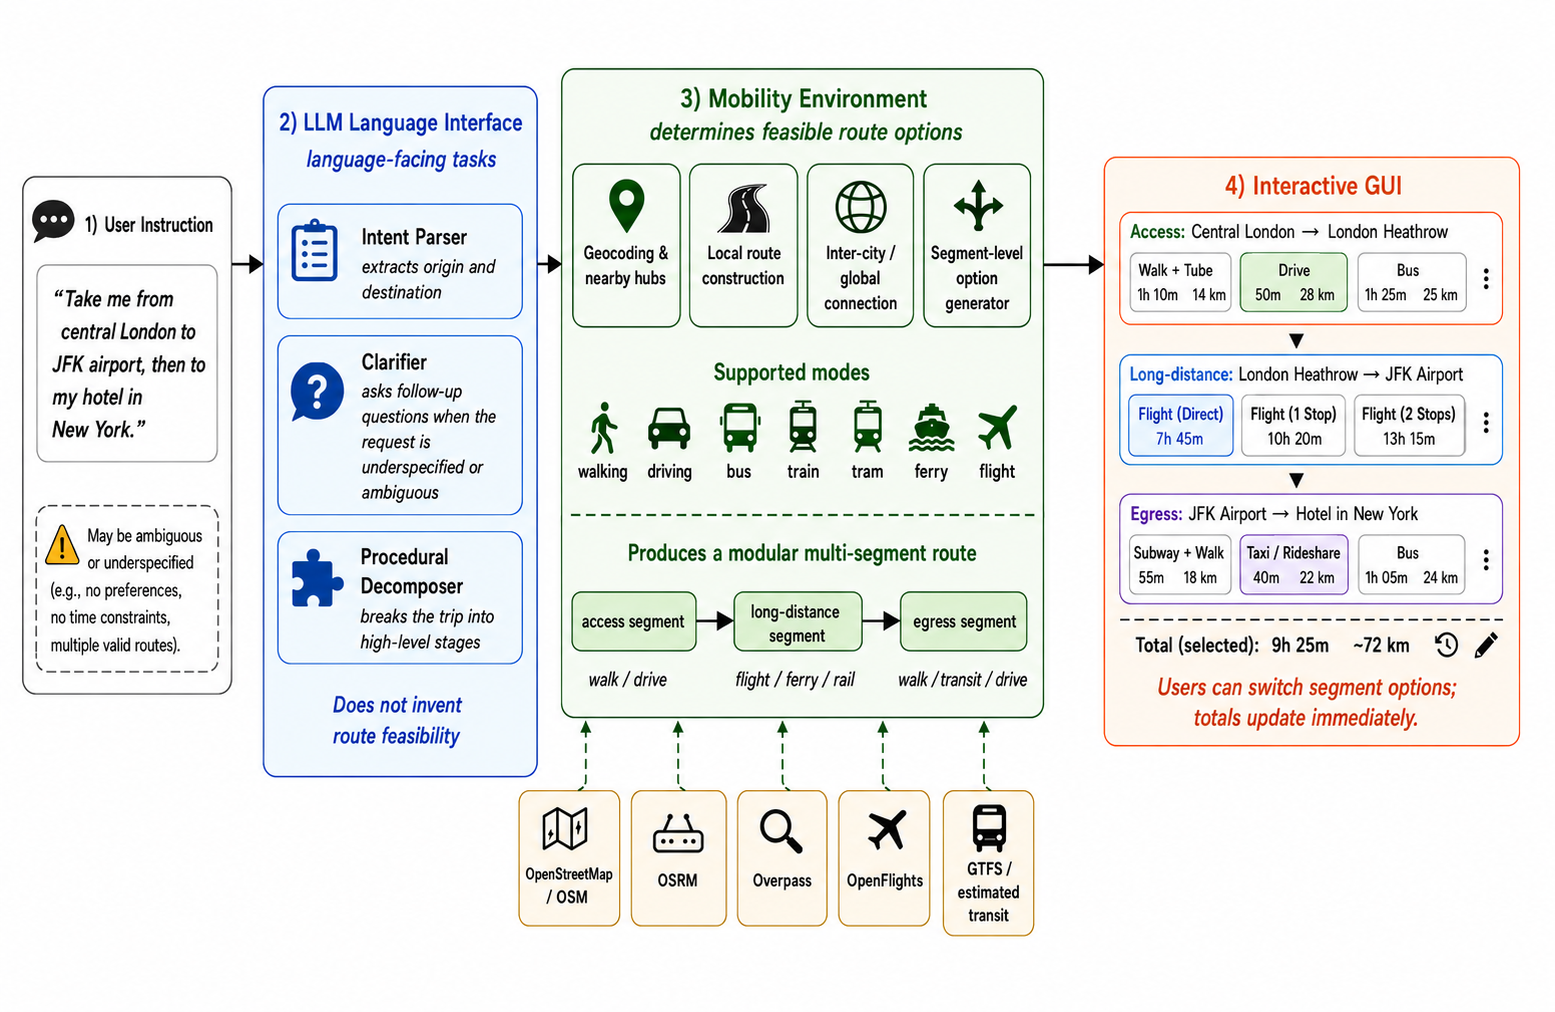
\includegraphics[width=\linewidth]{figure/pipeline2.png}
\caption{Overview of GLOBALNAV. GLOBALNAV converts a free-form user request into an environment-grounded multi-modal route. The LLM language interface performs intent parsing, ambiguity clarification, and route-option selection. The mobility environment grounds the resolved request in map and transportation evidence from OSM, OSRM, Overpass, OpenFlights, and transit resources, then constructs modular access, long-distance, and egress segments over walking, driving, public transit, ferry, and flight modes. The interactive GUI exposes alternative options for each segment and updates the selected total time and distance when users revise their choices.}
\label{fig:architecture}
\end{figure*}

\subsection{Language Interface}
The intent parser extracts the endpoint-level travel intent from a user instruction, including the origin, the final destination, and the clarification state of the request. Mode selection, transfer construction, and leg-level route planning are then handled by the routing environment rather than by the parser itself. When the user instruction is ambiguous or under-specified, such as ``take me to the airport from London,'' the clarifier identifies the unresolved part of the request and asks a follow-up question. For example, it may ask whether the user means Heathrow, Gatwick, Stansted, Luton, or London City Airport. The follow-up question is presented with candidate interpretations or destination options, allowing the user to resolve the ambiguity before route generation begins. Once the user answers, the system reparses the original instruction together with the clarification history and proceeds with the resolved travel intent.

\subsection{Environment-Grounded Route Generation}
The mobility environment grounds parsed endpoints in geographic and transportation data. It first geocodes the origin and destination with Nominatim~\citep{nominatim_2026} and then builds a modular travel solution. For local route requests, the solution can be represented as a single local segment. For inter-city or cross-region requests, the solution is composed of local access, long-distance connectivity, and local egress segments. For example, a global route may require traveling from the user's origin to a departure airport, flying to an arrival airport, and then continuing from the arrival hub to the final destination. When long-distance connectivity is required, the environment identifies relevant transportation hubs, such as airports, ports, or stations, for composing inter-city or cross-region travel. For each local segment, including local access and local egress, the current implementation returns:

\begin{itemize}[leftmargin=*]
\item one OSRM driving route;
\item up to five non-driving routes from graph search over walking, bus, train, and tram edges;
\item a pure walking route as a mandatory non-driving baseline.
\end{itemize}

For local route, the environment builds a local multi-modal graph from available routing and map data. The graph includes walking and driving connections, public-transport stops and route relations retrieved from OSM/Overpass, and short walking-transfer links between endpoints and nearby transit stops. The graph search ranks candidate paths by travel time while accounting for mode changes and transfer walks, producing alternatives such as direct walking, driving, bus access, train access, tram access, and mixed walk--transit routes. Long-distance connectivity is handled through transportation-hub evidence: air segments are grounded in OpenFlights airport and route connectivity, while ferry or maritime segments are grounded in map evidence such as ports and ferry terminals.

\subsection{Interactive Route Interface}

\begin{figure*}[t]
\centering
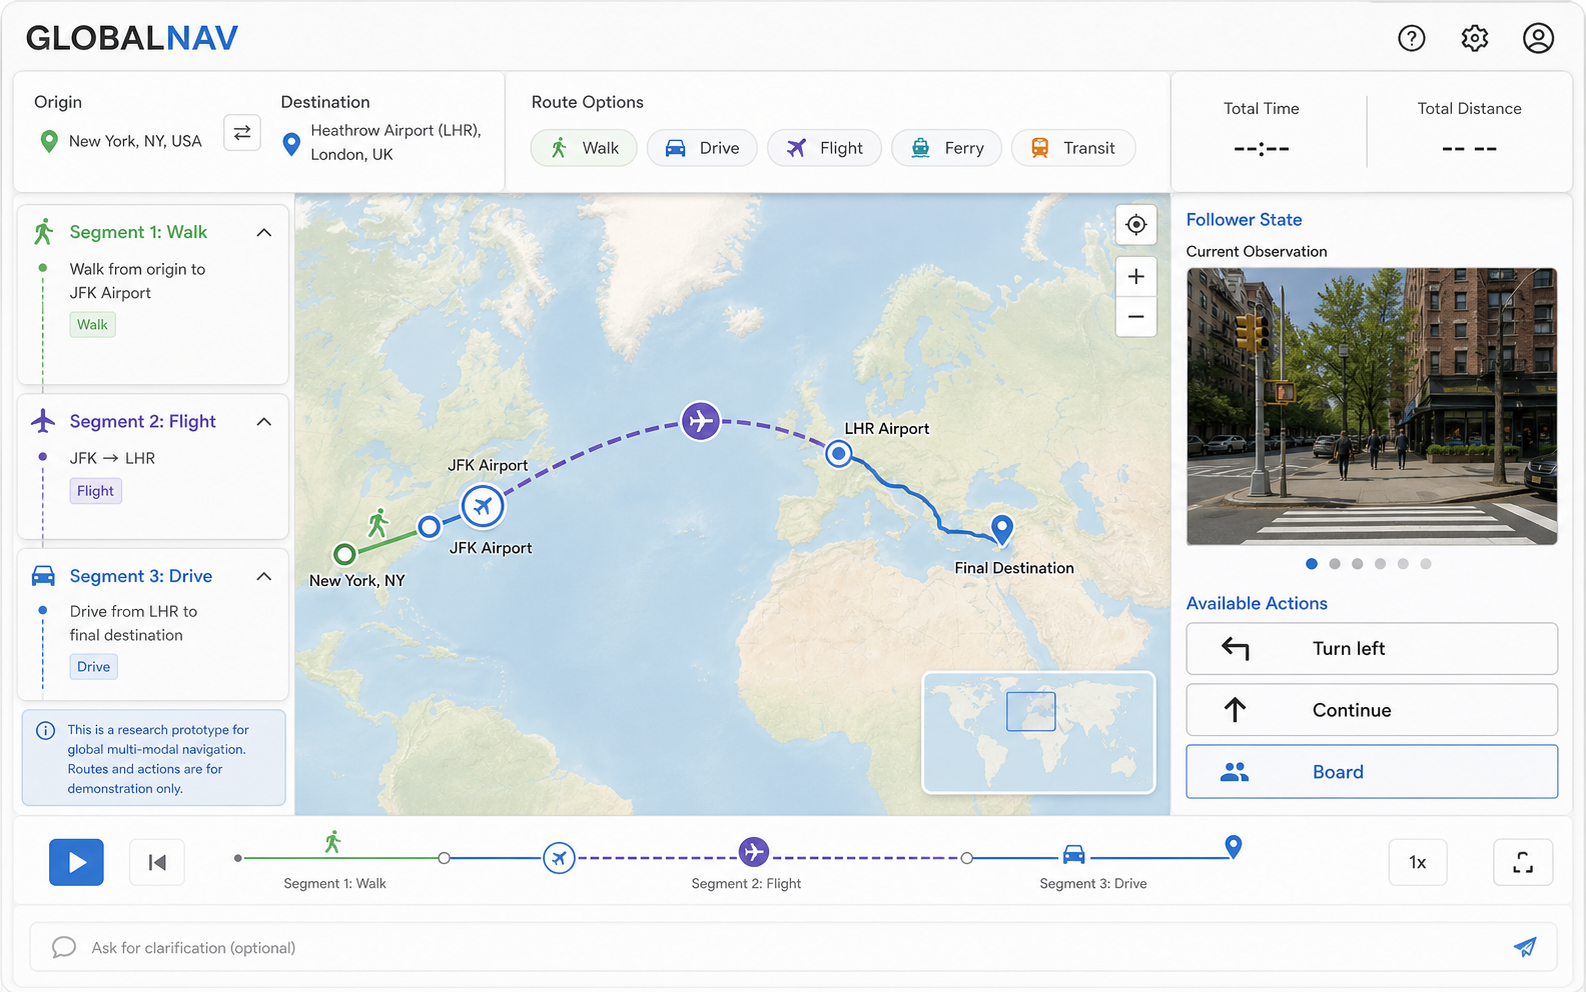
\includegraphics[width=\linewidth]{figure/demo.png}
\caption{Interactive \sys demo. The upper panel shows the system-parsed origin, destination, route preferences, and the total time and distance of the selected route. The left panel lists candidate options for each route segment, the bottom panel supports playback of the selected route, and the right panel displays street-view imagery according to the current playback position.}
\label{fig:demo}
\end{figure*}

Figure~\ref{fig:demo} shows the interface layout, including route segments, the map view, and the route playback panel. The interactive GUI presents each trip as a sequence of modular route segments, where each segment exposes multiple candidate options with visible travel time, distance, transportation mode, and micro-leg details. Users can switch the selected option for any segment, after which the total travel time, total distance, and displayed route geometry update immediately. After selecting a route, users can also inspect playback along the chosen path. For selected ground legs, the interface samples the route geometry into step-level nodes, derives headings and turn cues from the geometry, and can attach global street-view imagery when a provider is available.




\section{Evaluation}

First, we run a system-level demo evaluation on \bench, where each example tests whether the full pipeline resolves the user request, asks clarification questions when needed, grounds the final endpoints, and produces an environment-supported travel solution. Second, we evaluate \sys on additional route-request examples derived from existing dialogue and travel-query datasets to examine whether the same request-resolution procedure generalizes beyond \bench. Across both settings, we report endpoint-resolution and clarification metrics; SSR denotes the all-checks-passed success rate under the checks defined for each evaluation.

\subsection{GlobNav-Bench}

\bench is a compact 100-instruction evaluation set for testing the demo as a global multi-modal route-planning system. It covers local, regional, and global requests that require endpoint resolution, clarification, route grounding, and segment-level route options. The benchmark provides controlled examples for measuring whether \sys can resolve realistic travel requests and return grounded travel solutions.

\paragraph{Construction and Grounding.}
We begin from geographically diverse city and place seeds across North America, Europe, Asia, Oceania, Africa, South America, and the Middle East. The seed set includes hotels, landmarks, conference venues, campuses, museums, restaurants, transit-adjacent places, and other everyday points of interest, each recorded with a canonical name, geocoding query, coordinates, place type, and relevant map metadata. Starting from these seeds, we use \sys to instantiate same-city routes, hub-access routes, and inter-city or cross-region routes. We also add ambiguous or under-specified requests, such as missing origins, missing destinations, ambiguous place names, ambiguous airport references, and underspecified transport preferences.

\paragraph{Annotation and Validation.}
Human annotators review the environment-generated records. They verify endpoint correctness, correct or reject transfer points, check segment order, mark each leg's evidence status, and confirm that route options are meaningful alternatives rather than duplicates. Clarification examples are labeled with ask/no-ask decisions and ambiguity types, including missing origin, missing destination, ambiguous place name, ambiguous airport, and underspecified transportation preference.

A second annotator validates the final instruction, intent labels, clarification labels, route evidence, and segment structure.

\subsection{Metrics and Baselines}


\paragraph{Baselines.}
We include three baselines to isolate endpoint extraction and clarification behavior. The Rule-Based Parser is a deterministic non-dialogue parser that extracts origin and destination with hand-written templates, including patterns such as \textit{from X to Y}, \textit{departing from X}, and \textit{going to Y}, plus a small city and airport alias table. The NER Parser is an entity-only non-dialogue parser: it uses \texttt{dslim/bert-base-NER}~\citep{devlin-etal-2019-bert,huggingface_dslim_bert_ner_2026} to identify named entities, then assigns origin and destination with simple context rules or entity order. Neither parser performs clarification; any example that requires clarification is therefore counted as a failure. Because these parsers are not dialogue systems, Ask/Act and Target are not applicable. The No-clarification GPT-4.1 mini baseline uses the LLM parser but disables the clarification loop, forcing the system to parse and plan directly; this tests how much ambiguous instructions benefit from interaction.

\begin{table*}[ht]
\centering
\small
\setlength{\tabcolsep}{6pt}
\begin{tabular*}{\textwidth}{@{\extracolsep{\fill}}lrrrrr@{}}
\toprule
\textbf{Model} & \textbf{Ask/Act} $\uparrow$ & \textbf{Target} $\uparrow$ & \textbf{Origin} $\uparrow$ & \textbf{Dest.} $\uparrow$ & \textbf{SSR} $\uparrow$ \\
\midrule
Rule-Based Parser & \textsc{N/A} & \textsc{N/A} & 60.0 & 59.0 & 59.0 \\
NER Parser & \textsc{N/A} & \textsc{N/A} & 23.0 & 22.0 & 21.0 \\
No-clarification GPT-4.1 mini & 66.7 & \textsc{N/A} & 82.0 & 83.0 & 66.0 \\
\midrule
GPT-4.1 & 100.0 & 98.0 & 98.0 & 98.0 & 97.0 \\
GPT-4.1 mini & 100.0 & 97.5 & 98.0 & 98.0 & 97.0 \\
GPT-5 mini & 96.7 & 98.0 & 98.0 & 98.0 & 95.0 \\
Claude Sonnet 4.6 & 96.7 & 96.5 & 98.0 & 98.0 & 95.0 \\
GPT-5.4 mini & 96.7 & 95.0 & 96.0 & 98.0 & 94.0 \\
GPT-5.5 & 96.7 & 97.5 & 98.0 & 98.0 & 92.0 \\
Qwen2.5-7B-Instruct & 93.3 & 79.0 & 93.0 & 98.0 & 89.0 \\
Phi-3.5-mini-instruct & 96.7 & 84.5 & 95.0 & 96.0 & 79.0 \\
Gemini 2.5 Pro & 96.7 & 58.5 & 78.0 & 78.0 & 77.0 \\
Qwen2.5-3B-Instruct & 90.0 & 67.5 & 88.0 & 90.0 & 77.0 \\
Mistral-7B-Instruct-v0.3 & 86.7 & 59.5 & 84.0 & 94.0 & 74.0 \\
Qwen2.5-1.5B-Instruct & 50.0 & 77.0 & 91.0 & 95.0 & 21.0 \\
Qwen2.5-0.5B-Instruct & 33.3 & 45.0 & 86.0 & 83.0 & 0.0 \\
\bottomrule
\end{tabular*}
\caption{System-level success on all 100 \bench instructions. \textbf{SSR} is the all-checks-passed system success rate: the request must be resolved, any required clarification must be handled correctly, and the final origin and destination must match the annotation. \textsc{N/A} indicates metrics that are undefined for non-dialogue baselines. OpenAI mini models are included as lower-cost alternatives to their full-size counterparts.}
\label{tab:system}
\end{table*}

\begin{table*}[ht]
\centering
\small
\setlength{\tabcolsep}{6pt}
\begin{tabular*}{\textwidth}{@{\extracolsep{\fill}}lrrrrr@{}}
\toprule
\textbf{Dataset} & \textbf{Ask/Act} $\uparrow$ & \textbf{Target} $\uparrow$ & \textbf{Origin} $\uparrow$ & \textbf{Dest.} $\uparrow$ & \textbf{SSR} $\uparrow$ \\
\midrule
MultiWOZ 2.4 & 99.0 & 98.1 & 99.2 & 99.2 & 98.2 \\
SGD & 99.7 & 97.3 & 96.5 & 96.2 & 95.8 \\
ATIS & 99.8 & -- & 99.2 & 99.3 & 98.4 \\
\midrule
Overall & 99.4 & 98.0 & 98.4 & 98.4 & 97.4 \\
\bottomrule
\end{tabular*}
\caption{External OD parsing and clarification results using GPT-4.1 mini (\%, full eligible pool, 1,723 examples). Metrics follow Table~\ref{tab:system}. \textbf{Target} is measured only on native clarification examples; ATIS has no such examples in this evaluation. Overall SSR is 1,678/1,723.}
\label{tab:external_od}
\end{table*}

\paragraph{Metrics}
We report four component metrics and an overall system success rate. \textbf{Ask/Act} measures whether the system makes the correct dialogue decision: answering directly for complete requests or asking a clarification question for under-specified requests. \textbf{Target} is evaluated on clarification examples and measures whether the follow-up question targets the missing endpoint. \textbf{Origin} and \textbf{Dest.} measure whether the final resolved origin and destination match the annotation. \textbf{SSR} is the system-level success rate for the complete route-planning demo: a run succeeds only when the system resolves the user intent, handles clarification when needed, grounds the endpoints in map data, and passes all required endpoint and clarification checks for that example.

\subsection{Implementation Details.}
The \sys system-level experiment is evaluated on the full set of 100 instructions. Each example includes verified route evidence, gold origin and destination entities, ask/no-ask clarification labels, and ambiguity types. We evaluate recent closed-source LLMs including GPT-5.5, GPT-5.4 mini, GPT-5 mini, GPT-4.1, GPT-4.1 mini~\citep{openai_models_2026}, Claude Sonnet 4.6~\citep{anthropic_sonnet46_2026}, and Gemini 2.5 Pro~\citep{google_gemini_models_2026}, as well as open-weight models including Qwen2.5~\citep{yang2024qwen25technicalreport}, Phi-3.5-mini-instruct~\citep{abdin2024phi-}, and Mistral-7B-Instruct-v0.3~\citep{jiang2023mistral7b}. All LLM-based systems use the same parsing and clarification prompts. In the deployed demo, GPT-4.1 mini is used as the default model since it offers a practical balance of low latency, low cost, and high accuracy, reaching 97\% SSR in Table~\ref{tab:system}. Unless otherwise specified, decoding uses temperature 0, and each example is run once.

For intent resolution, an origin or destination is correct if it matches the annotated canonical entity after geocoding; when only coordinates are available, we use distance thresholds by entity type: 100 meters for POIs and buildings, 1 km for airports, stations, and ports, and the annotated administrative area or 10 km from the city center for city-level endpoints. For ambiguous examples, clarification resolution is counted as success only when the system asks an appropriate follow-up question and the resolved intent matches the gold annotation.

\paragraph{Purpose.}
The system-level experiment evaluates the complete demo on \bench. To test the deployable language-facing component at larger scale, we additionally evaluate the parser and clarification loop on OD-eligible subsets derived from existing datasets: MultiWOZ 2.4~\citep{ye-etal-2022-multiwoz}, Schema-Guided Dialogue (SGD)~\citep{rastogi-etal-2020-schema}, and ATIS~\citep{hemphill-etal-1990-atis}. This experiment isolates OD intent resolution and clarification behavior rather than route construction.

\paragraph{Data and protocol.}
We do not evaluate the full original datasets; instead, we use the full OD-eligible subsets recovered from their native annotations. MultiWOZ 2.4 contributes 381 taxi/train examples: 225 explicit OD turns (205 train, 20 taxi) and 156 native clarification examples (140 train, 16 taxi). SGD contributes 733 examples from the Buses\_3, Flights\_4, and Trains\_1 services: 332 explicit OD turns and 401 native clarification examples. ATIS contributes 609 single-turn explicit flight queries and no clarification examples. For MultiWOZ and SGD, explicit examples come from original user turns that contain both origin and destination information, while clarification examples come from original incomplete user turns followed by the dataset's next user answer. The \texttt{expected\_clarification} label is not a native field; it is deterministically derived from native dialogue state, dialogue acts, or BIO slot annotations by checking whether the first user-visible request already contains both OD endpoints. During evaluation, the system first receives only the initial user request. If and only if it asks the correct type of clarification question (missing origin vs. missing destination), the evaluator supplies the original next user answer before scoring the final parse.

\subsection{Results and Error Analysis}



Table~\ref{tab:system} shows that GPT-4.1 and GPT-4.1 mini obtain the strongest system-level results on \bench, both reaching 97\% SSR. GPT-5 mini and Claude Sonnet 4.6 follow at 95\%, and Qwen2.5-7B-Instruct is the strongest open-weight model at 89\%. The rule-based, NER, and no-clarification baselines are substantially weaker, indicating that robust endpoint resolution and targeted clarification are important for the demo.

Table~\ref{tab:external_od} shows similarly strong results on the external route-request examples: GPT-4.1 mini reaches 97.4\% SSR over 1,723 examples, with 99.4\% Ask/Act accuracy and 98.4\% accuracy for both origin and destination. The remaining failures are mostly endpoint-resolution or clarification errors, such as unnecessary or missed clarifications, wrong clarification targets, and endpoint reversals.

\section{Conclusion}

We introduced \sys, an environment-driven global multi-modal route-planning demo for travel requests that span local access, long-distance movement, transfers, and ambiguous endpoints. \sys uses the LLM as a language interface for intent resolution and clarification, while endpoint grounding and route construction are handled by an external mobility environment. The evaluation shows that this design resolves most \bench requests and generalizes to OD-like examples from MultiWOZ 2.4, SGD, and ATIS. Overall, \sys and \bench provide a compact testbed for grounded, language-driven global navigation beyond single-city or single-mode route planning.

\section*{Limitations}

\sys does not download a complete global map.
It queries route and map data on demand and caches results.
This makes the demo lightweight but dependent on API availability and coverage. OpenFlights only provides connectivity, not real-time schedules or ticket availability. Public-transit, ferry, and rail coverage depends on available public evidence; when schedules are unavailable, these modes are reported through route evidence and mode-chain coverage rather than timetable duration.

\bibliography{references}





\clearpage
\appendix

\section{Prompt and Evaluation Details}
\label{sec:prompts}

\paragraph{Intent parsing prompt.}
The deployed parser is constrained to extract origin and destination only. It is instructed not to plan routes or choose transport modes, and to set \texttt{needs\_clarification=true} only when an endpoint is genuinely missing or ambiguous. The system prompt in \texttt{globe\_nav/llm\_parser.py} is shown below, with line breaks added for print layout; non-ASCII examples in the code are rendered with their English equivalents for pdfLaTeX compatibility:
\begin{lstlisting}[style=promptstyle]
You parse travel instructions into
origin and destination ONLY.

Do NOT plan routes or choose transport modes --
the navigation environment does that.

Rules:
1. Extract the most specific origin and
   destination place names.
2. Set needs_clarification=true ONLY
   when origin or destination is
   genuinely missing or ambiguous.
3. Do NOT ask about airports if the user
   already named one (e.g. Sydney Airport, SYD).
4. Do NOT ask about university campus if the user
   already named one (e.g. University of Liverpool).
5. Procedural waypoints (central station,
   facing direction) are NOT ambiguities --
   ignore them for clarification.
6. Return valid JSON only.

JSON schema:
{
  "origin": "full place name; city/country if known",
  "destination": "full place name; city/country if known",
  "needs_clarification": false,
  "questions": [
    {
      "category": "snake_case_id",
      "question": "question text",
      "options": ["opt1", "opt2"]
    }
  ]
}
\end{lstlisting}
The user message template is:
\begin{lstlisting}[style=promptstyle]
User instruction:
{instruction}
\end{lstlisting}

\paragraph{Clarification prompt.}
Clarification is implemented as a one-turn loop over the same parser rather than as a separate LLM prompt. The system stores the category and text of the question, appends the user's answer to a clarification history, and reparses the original instruction with that history:
\begin{lstlisting}[style=promptstyle]
User instruction:
{instruction}

Clarification history:
Q ({category}): {question}
A: {answer}
\end{lstlisting}
The evaluation supplies a gold answer only when the system asks for the gold missing endpoint.

\paragraph{Route-option selection prompt.}
When the interface needs a default option for each route segment, the recommender in \texttt{globe\_nav/planner/recommender.py} asks the LLM to select among environment-generated candidates rather than invent new routes:
\begin{lstlisting}[style=promptstyle]
Pick one default option_id per segment for this trip.
Prefer realistic choices: drive/taxi to airport,
valid flights, train/bus for last mile
when available. Return JSON:
{"selections": {"segment_id": "option_id", ...}}
\end{lstlisting}
The user message template is:
\begin{lstlisting}[style=promptstyle]
{
  "trip": "{origin} -> {destination}",
  "segments": [
    {
      "segment_id": "{segment_id}",
      "title": "{segment_title}",
      "type": "{segment_type}",
      "options": [
        "{option_id}: {label} ({minutes}min)"
      ]
    }
  ]
}
\end{lstlisting}

\end{document}
